\section{General-purpose Counterfactuals}
\label{sec:general_purpose}



\newcommand{\tagdefine}[1]{\emph{{\color{darkgray}#1} }}
%\renewcommand{\arraystretch}{1.1}
\newcommand{\TagTable}{
\begin{table*}
\small
\centering
\begin{tabular}{@{} p{0.11\linewidth} p{0.61\linewidth} p{0.22\linewidth} @{}}
\toprule
\textbf{\Tagstr} & \textbf{Definitions and \sysname-generated Examples} & \textbf{Training Datasets} \\ 
\midrule
\ctrltag{negation}
 & A dog is \add{not} embraced by the woman.
 &\cite{kaushik2019learning}
\\ \midrule
\ctrltag{quantifier}
 & \swap{A dog is}{Three dogs are} embraced by the woman. 
 &\cite{gardner2020contrast}
\\ \midrule
\ctrltag{shuffle}
 & \tagdefine{To move (or swap) key phrases or entities around the sentence.} \newline
 A \swap{dog}{woman} is embraced by the \swap{woman}{dog}.
 &\cite{zhang2019paws}
\\ \midrule
\ctrltag{lexical}
 & \tagdefine{Ro change just one word or noun chunks without breaking the POS tags.} \newline
 A dog is \swap{embraced}{attacked} by the woman.
 &~\cite{sakaguchi2019winogrande}
\\ \midrule
\ctrltag{resemantic}
 & \tagdefine{To replace short phrases or clauses without affecting the parsing tree.}\newline
 A dog is \swap{embraced by the woman}{wrapped in a blanket}.
 &\cite{wieting2017paranmt}
\\ \midrule
\ctrltag{insert}
 & \tagdefine{To add constraints without affecting the parsing structure of other parts.} \newline
 A dog is embraced by the \add{little} woman.
 &\cite{mccoy2019right}
\\ \midrule
\ctrltag{delete}
 & \tagdefine{To remove constraints without affecting the parsing structure of other parts.} \newline
 A dog is embraced \remove{by the woman}.
 &~\cite{mccoy2019right}
\\ \midrule
\ctrltag{restructure}
 & \tagdefine{To alter the dependency tree structure, \eg changing from passive to positive.} \newline
 A dog is \swap{embraced by}{hugging} the woman.
 &\cite{wieting2017paranmt}
\\
\bottomrule
\end{tabular}
\vspace{-5pt}
\caption{
We design a list of \tagstrs to drive the generation.
We show their \emph{\sysname-generated} examples, and the representative training datasets for the corresponding patterns. 
Details are in Appendix~\ref{appendix:train_data}.
%More examples are in Appendix~\ref{appendix:example}.
}
%\wts{Change all the examples to be on an identical sentence, not all different cases. And consider further annotate the tags based on whether they just do semantic change or also syntactic change.}}
\label{table:ctrltag}
\vspace{-5pt}
\end{table*}
}
% on a particular instance
% 
\subsection{Definition and Desiderata}
\label{sec:desiderata}


Given an instance $x \in \xset$, a generator $g$ produces a set of counterfactuals $\hat{\xset} = \{\xp_1, \xp_2, ...\}$ with various relationships $x \veryshortarrow \xp_i$. % (referred as $\relation{\xp_i}$ for simplicity).
% Each $\xp_i$ perturbs $x$ with certain strategies like negations, syntactic restructuring, etc., and the edited spans are instantiations of the strategies.
For example, \swap{great}{not great}, \swap{kids}{no one} in Figure~\ref{fig:teaser}B are both instances of the \ctrltag{negation} relationship.
% The importance of certain $\relation{\xp}$ changes along with applications.
Each $(x, \xp)$ pair shares multiple relationships --- these two are also instances of the \emph{label flipping} relationship if the task is sentiment analysis (but might not be for other tasks).
As illustrated in \S\ref{sec:intro}, knowing which relationships apply aids selection for downstream applications.

We expect $g$ to produce counterfactuals $\xp$ that are (1) \textbf{close} to $x$, preferably only involving the minimal changes necessary to establish a certain effect~\cite{pearl2018causal}, allowing users to make causality assessments.
The generated $\xp$ should also be (2) \textbf{fluent}, \ie grammatically correct~\cite{morris2020textattack} and semantically meaningful (\eg \exinline{Colorless green ideas sleep furiously} is not meaningful~\cite{chomsky2002syntactic}).
Fluency operationalizes ``probable'' counterfactuals in the context of NLP;
as \citet{kahneman} stated, humans strongly favor counterfactuals that are close to the original instance, but also prefer those that could have easily happened without assuming rare events or strange coincidences.
%Humans strongly favor counterfactuals that are close to the original instance, but also prefer them to be probable, \ie they could have easily happened without assuming rare events or strange coincidences~\cite{kahneman}.
%We operationalize ``probable'' in the context of NLP by requiring $g$ to generate (2) \textbf{fluent} $\xp$, \ie grammatically correct~\cite{morris2020textattack} and semantically meaningful (\eg \exinline{Colorless green ideas sleep furiously} is not meaningful~\cite{chomsky2002syntactic}).
Further, as a general-purpose generator, $g$ should produce counterfactuals with a measure of (3) \textbf{control} over relationships $x \veryshortarrow \xp$,  %$\relation{\xp}$,
such that the counterfactuals can vary with the object-of-attention in each application (the ``focus rule''~\cite{kahneman}).
Finally, %even though infinite diverse counterfactuals can be produced~\cite{pearl2018causal},
we expect $g$ to output a (4) \textbf{diverse} set of $\xp$ in terms of relationships, covering a large variety of ``what-ifs'' for different applications~\cite{pearl2018causal}.

%A counterfactual $\xp$ should be \textbf{close} to $x$, preferably only involving the minimal changes necessary to establish a certain effect~\cite{pearl2018causal} for causality assessments about $\relation{\xp}$. 
%Humans strongly favor counterfactuals that are close to the original instance~\cite{kahneman}, while also being probable, \ie which could have easily happened without assuming rare events or strange coincidences.
%We operationalize ``probable'' in the context of NLP by requiring $\xp$ that are \textbf{fluent}, \ie grammatically correct~\cite{morris2020textattack} and semantically meaningful (\eg \exinline{Colorless green ideas sleep furiously} is not meaningful~\cite{chomsky2002syntactic}).
%A general-purpose generator should be able to generate counterfactuals with a measure of \textbf{control} over relationships $\relation{\xp}$, such that counterfactuals vary with the object of attention depending on the application at hand (the ``focus rule''~\cite{kahneman}).
%Finally, we expect the output set $\hat{\xset}$ to be \textbf{diverse} in terms of relationships, so as to support diverse applications.

% Meanwhile, we also expect to collect sets with (4) \textbf{controlled} $\relation{\xp}$ relationships.
% The control is essential to support a wide range of specific applications, \eg counterfactual explanations on salient features (\S\ref{sec:app_explain}), error analyses that group semantically or syntactically related $\xp$ (\S\ref{sec:app_err_analysis}), etc.
% It reflects the ``focus rule''~\cite{kahneman}: counterfactuals would vary with the object of attention.
%, even when the same variable is acted upon.
%Following common practice in NLP research, we estimate \emph{closeness} using the semantic and syntactic distance between $x$ and $\xp$~\cite{morris2020textattack, madaan2020generate}.
% However, $\xp$ also needs to be (2) \textbf{fluent}, \ie grammatically correct~\cite{morris2020textattack} and semantically meaningful (\eg \exinline{It's scary for water} is not meaningful.)
% This estimates the likelihood of a sentence occurring in reality; as \citet{kahneman} stated, the counterfactual scenario should be one that could have easily happened without rare assumptions. 
%In NLP, this translates to sentences that are likely to be written.


%However, $\xp$ also needs to be realistic, \ie the counterfactual scenario should be one that could have easily happened, without rare assumptions or coincidences~\cite{kahneman}. 
%In NLP, this translates to sentences that are likely to be written, \ie (2) \emph{fluent} counterfactuals that are grammatically correct~\cite{morris2020textattack} and semantically meaningful (\eg \exinline{It's scary for water} is grammatically correct but not meaningful.) 

% Since there can be an infinite number of ``what-ifs''~\cite{pearl2018causal}, we also consider properties of $\hat{\xset}$, the produced \emph{set of counterfactuals}.

% Since our goal is to produce a general-purpose set of counterfactuals, we expect the set to be (3) \textbf{diverse} in terms of relationships between $x$ and $\xp$.
%However, when the targeted relationship is unclear, an approximation could be the similarity of counterfactuals \emph{to each other} (using \eg self-BLEU~\cite{Hu2017TowardCG}).
%, and also to contain various instantiations of the same relationship.
% Meanwhile, we also expect to collect sets with (4) \textbf{controlled} $\relation{\xp}$ relationships.
% The control is essential to support a wide range of specific applications, \eg counterfactual explanations on salient features (\S\ref{sec:app_explain}), error analyses that group semantically or syntactically related $\xp$ (\S\ref{sec:app_err_analysis}), etc.
% It reflects the ``focus rule''~\cite{kahneman}: counterfactuals would vary with the object of attention.
%Additionally, augmentations usually prioritize (3) \emph{diversity} --- a group of $x$s are preturbed using various strategies, and various initiations under the same strategy, such that they provide different constraints on finetuning decision boundaries.
%On the other hand, evaluations and explanations require more (4) \emph{controlled} perturbations for systematic and targeted inspections.
%The diversity and the controllability are two competing factors, and prior work focusing on certain applications follow one of two extremes.
%Those that thrive in diversity are either too uncontrolled (\eg text generation~\cite{iyyer2018adversarial}) or hard to scale (\eg manual rewrites~\cite{kaushik2019learning, gardner2020contrast}), whereas those that rely on templates or heuristic rules usually only cover limited linguistic patterns~\cite{li2020linguistically}.
\TagTable


\begin{figure}[t]
\centering
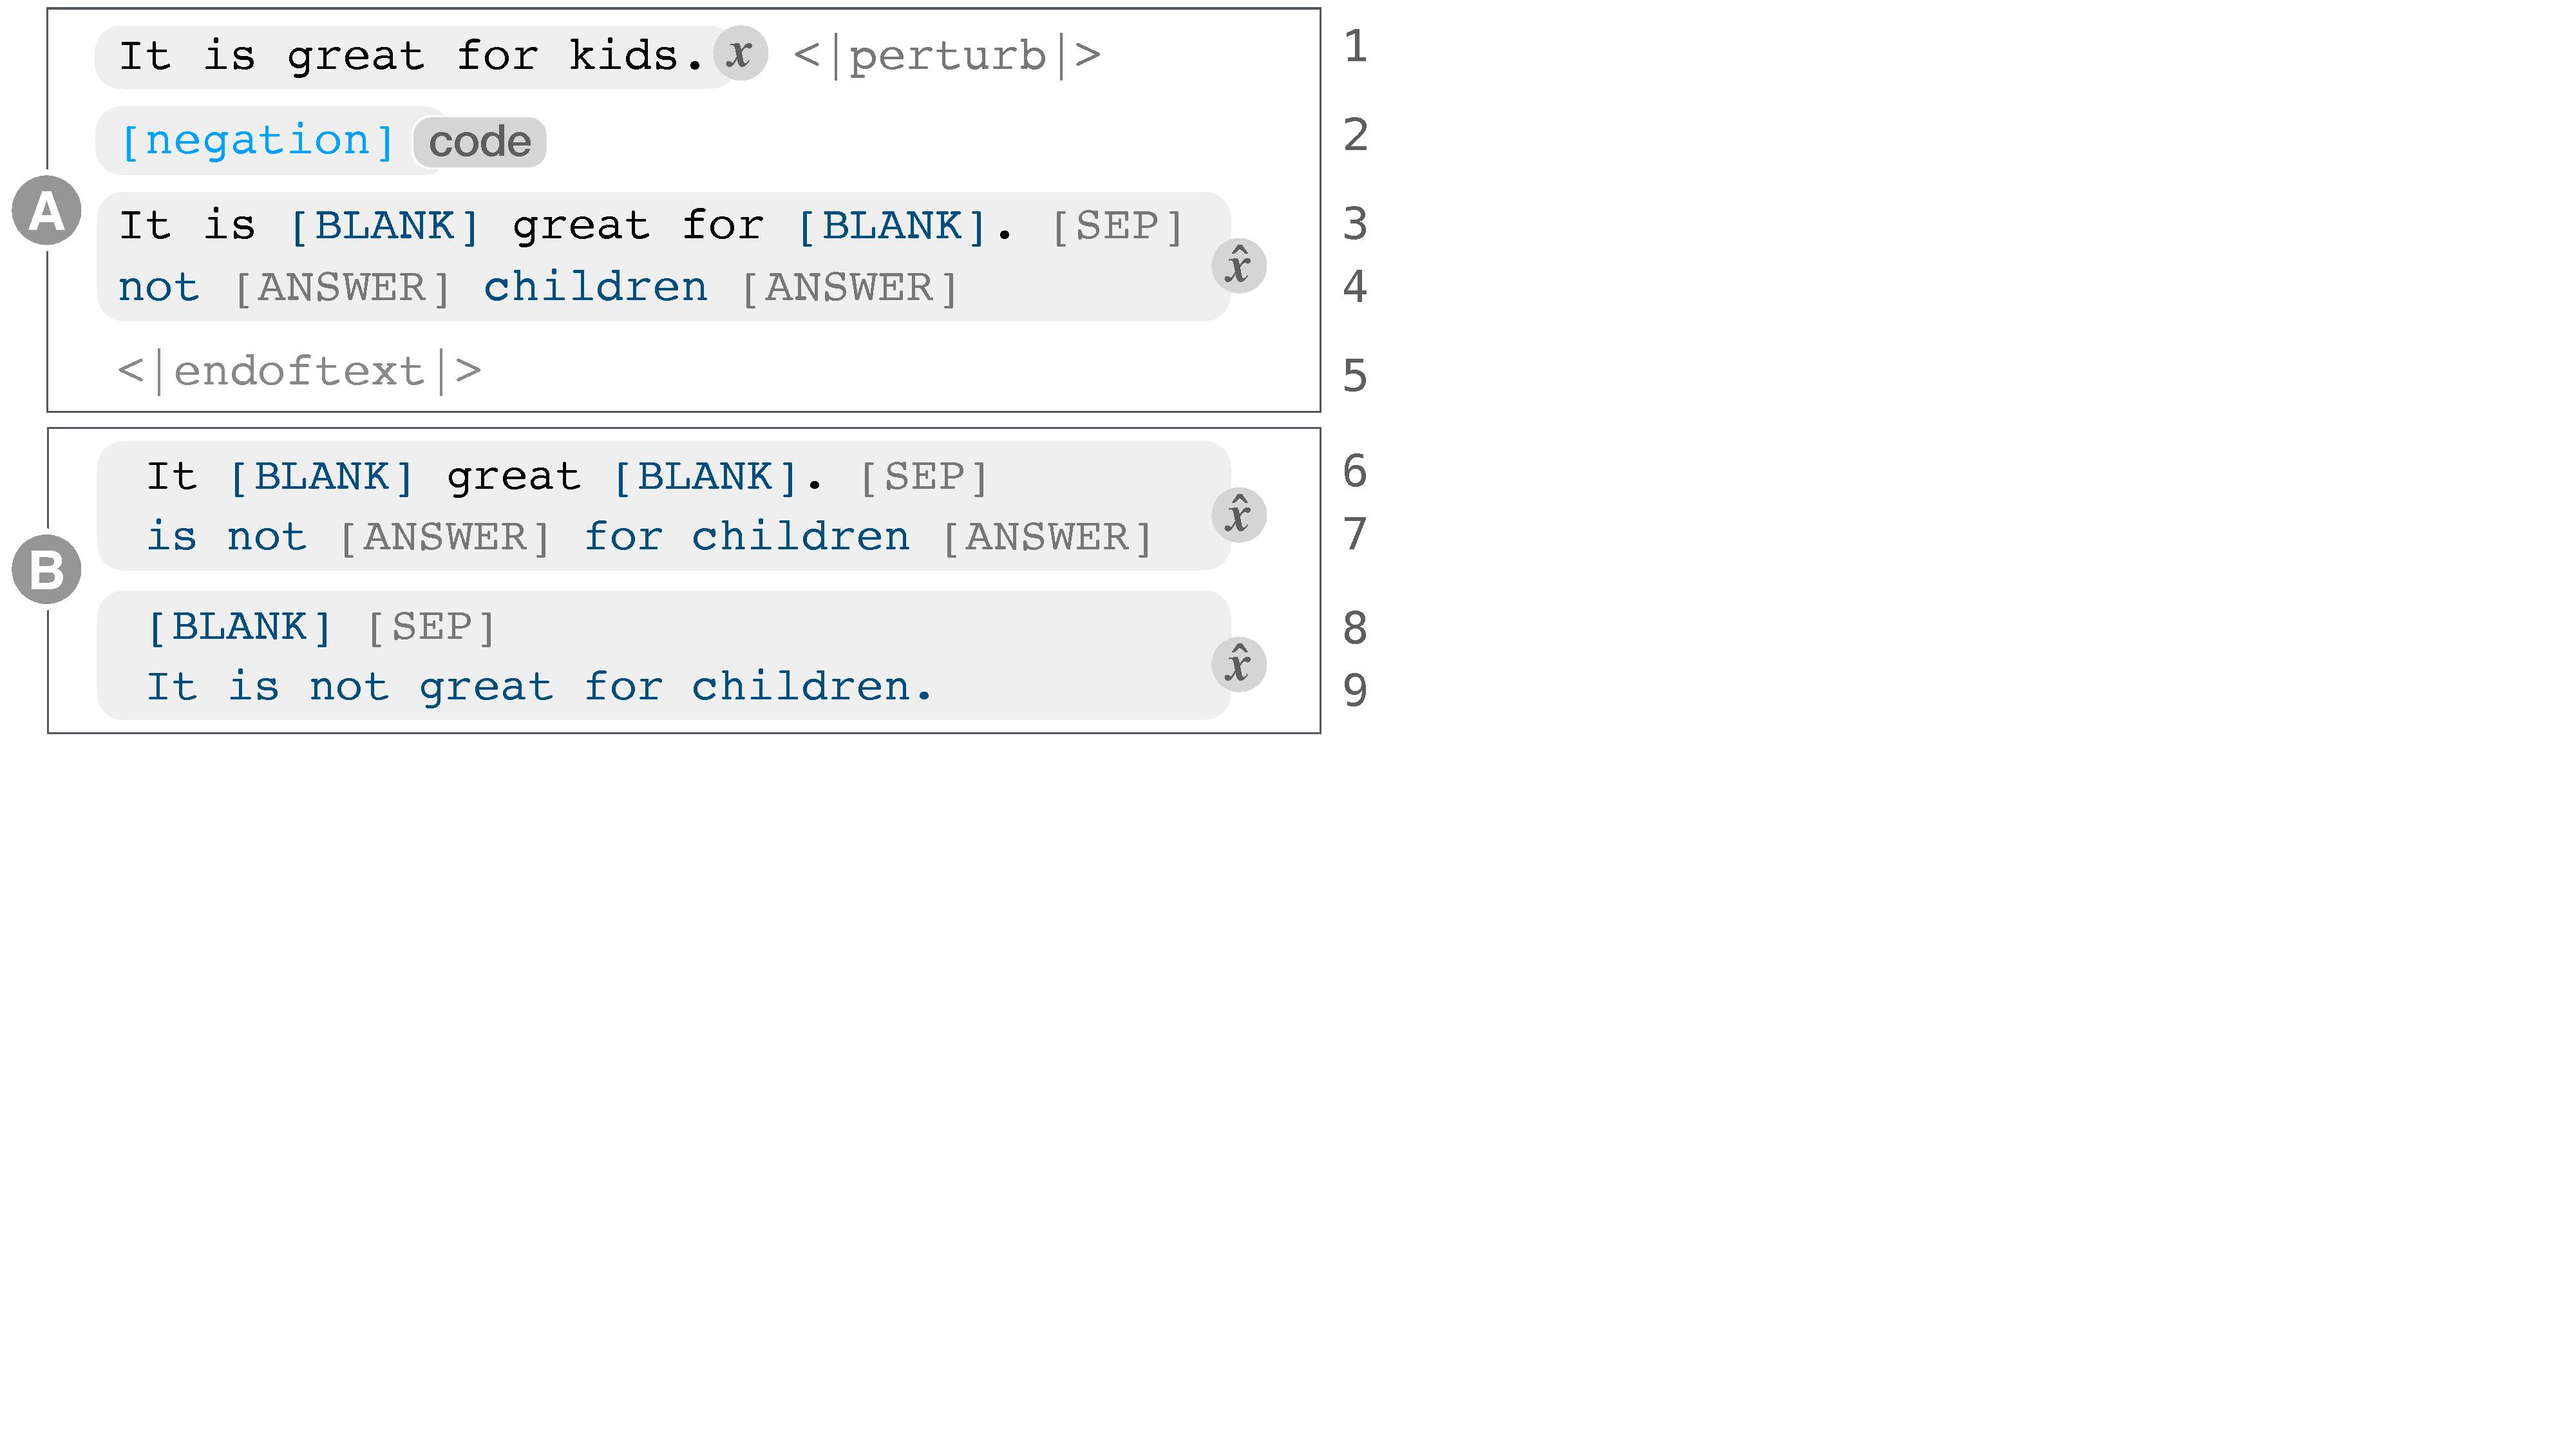
\includegraphics[trim={0 18.6cm 31.5cm 0cm}, clip, width=1\columnwidth]{figures/blank.pdf}
\vspace{-15pt}
\caption{ 
(A) \sysname prompt format, which concatenates the original $x$, the \tagstr, and the $\xp$ (\exinline{It is not great for children} converted to the infilling structure).
At \emph{generation} time, \sysname accepts prompts that just include $x$ (Line 1), or optionally with the \tagstrshort and the \texttt{[BLANK]}s (Lines 2--3), and fill in the blanks sequentially with spans separated by \texttt{[ANSWER]}s (Line 4).
%During training, the \tagstrshorts and blanks are automatically extracted.
(B) \sysname allows blanking at different granularities (even the entire sentence), such that Lines 3--4 in (A) can be replaced by Lines 6--7 or 8--9. 
%\dq{}
%We get multiple training texts per pair, by blanking $\xp$ subtrees that contain the change, or the entire sentence.
}
\vspace{-10pt}
\label{fig:blank}
\end{figure}


\subsection{Conditional Counterfactual Generation}
\label{subsec:nlg}



We frame counterfactual generation as a conditional text generation task using language models (LMs). To ensure that $\xp$ is \emph{close} to $x$ rather than arbitrary text, we condition the generation on $x$, followed by a special token (Line 1 in Figure~\ref{fig:blank}A).
In Line 2, we have \emph{\tagstrs} \cite{ctrl} such as \ctrltag{negation}.
We design them to specify types of perturbation from among lexical, syntactic, or semantic aspects (see Table \ref{table:ctrltag}), inspired by prior work that categorizes manually created counterfactuals~\cite{kaushik2019learning, gardner2020contrast}.
% All the \tagstrshorts are described in Table~\ref{table:ctrltag}. 
As an additional layer of control over $x \veryshortarrow \xp$, % $\relation{\xp}$,
we allow users to specify \emph{where} changes happen by having the LM infill \texttt{[BLANK]} tokens~\cite{donahue2020enabling}, rather than generating arbitrary counterfactuals (Lines 3--4).
At generation time, if the user provides only the original example, \sysname will generate the \tagstr, the location of blanks, and the infilling (Lines 2--4). 
Alternatively, the user can specify the \tagstr, or the \tagstr \emph{and} the location of the blanks, to exercise different degrees of control depending on the application.

% \paragraph{\emph{Closeness} and \emph{Controllability}: Conditional text generation.}
%1. We frame it as conditional text generation. We always condition on the original x (Line 1)
%2. Control codes: explain what they are , reference table 1, etc (Line 2)
%3. Blanking: we extend ILM, etc. This is why it's nice, etc (Line 3).
%4. Control codes & blanking allow for control, but they are optional: the generator can generate them based on the original x

% We frame counterfactual generation as a conditional text generation task using language models (LMs), and wrap the \emph{conditions} into textual prompts as in Figure~\ref{fig:blank}.
% First, to ensure $g$ generates $\xp$ that are \emph{close} to $x$ (rather than arbitrary text), we build mappings between paired, and always condition the generation on the original $x$ (Line 1).

% Second, to achieve the control on $\relation{\xp}$, we include \emph{\tagstrs} (\eg \ctrltag{negation} in Line 2), which encode the type of perturbations.
% Inspired by prior work categorizing manually created counterfactuals~\cite{kaushik2019learning, gardner2020contrast}, we design eight \tagstrshorts (Table~\ref{table:ctrltag}) that distinguish lexical, syntactic, and semantic perturbations.

% Besides the perturbation types, we additionally control where changes happen.
% We extend the Infilling by Language Modeling (ILM) framework~\cite{donahue2020enabling}, such that $\xp$ contains \texttt{[BLANK]} tokens where perturbations are to be applied (Line 3). 
% As shown in Figure~\ref{fig:blank}B, Lines 6--9, ILM allows for perturbations of any length (additions and deletions) beyond single word substitutions.

% At generation time, with Line 2 and 3 specified, \sysname can just fills in the blanks sequentially according to the controls (Line 4).
% However, the control conditions are optional.
% When we exclusively condition the generation on $x$ (Line 1), \sysname can generate Line 2--3 on its own by sampling the \tagstr and the location of blanks.

To train a conditional model, we combine six existing sentence-pair datasets, each containing a subset of the desired phenomena in Table~\ref{table:ctrltag}. 
Further, we find naturally occurring sentence pairs (filtered by edit distance to guarantee closeness) in non-paired datasets including CommonGen~\cite{lin-etal-2020-commongen}, Natural Questions~\cite{kwiatkowski-etal-2019-natural}, and SQuAD~\cite{rajpurkar-etal-2016-squad}, such that the resulting dataset contains \emph{diverse} counterfactuals.\footnote{We exclude data related to our applications, \eg PAWS-QQP \cite{zhang2019paws}. }
%(details in Appendix~\ref{appendix:train_data}). 
We translate each $(x, \xp)$ in the dataset into the format given in Figure~\ref{fig:blank}A, by computing the \tagstr from syntactic features (POS tags and dependency trees), and placing \texttt{[BLANK]}s in $\xp$. 
To allow flexible blanking at generation time, we create multiple prompts per pair that cover  different dependency tree structures related to the perturbed spans (Figure~\ref{fig:blank}B), resulting in $657,144$ prompts from $186,451$ pairs.
% we train gpt-2 on this and add filtering

We train \sysname by finetuning GPT-2~\cite{radford2019language} on the resulting prompts (other LMs could also be used).
While the original GPT-2 produces \emph{fluent} text, some combinations of \tagstrs and blanks cause \sysname to generate nonsensical results.
Following \citet{morris2020textattack}, we score both $x$ and $\xp$ with GPT-2, and filter $\xp$ when the log-probability (on the full sentence or the perturbed chunks) decreases more than 10 points relative to $x$.
Fully automated uses of \sysname (\eg adversarial attacks) may benefit from stricter constraints, at the cost of diversity --- more surprising changes may be filtered even if they are fluent.


\subsection{Intrinsic Evaluation}
\label{subsec:intrinsic}



We verify the \emph{fluency} for \sysname counterfactuals in three tasks/datasets: (1) \sst Analysis, \dsst~\cite{socher2013recursive},
(2) Natural Language Inference (\nli), \dnli~\cite{bowman-etal-2015-large}, and 
(3) Duplicate Question Detection (\dqqp)~\cite{wang2018glue}.
We randomly select 100 sentences per dataset, generate 3 $\xp$ per $x$, and ask crowd workers to rate whether they are \emph{``likely written by native speakers.''}
The workers rated most counterfactuals as fluent: $78\%$ for \dsst, $76\%$ for \dqqp, and $86\%$ for \dnli. In subsequent sections, we show these rates are suitable for applications where people ``team up'' with \sysname.
% One of the authors also manually labeled counterfactuals of 120 instances, and arrived at similar fluency.
% Without automatic filtering, the fluency rate decreases to $61\%$.

Further, we quantify the impact of \tagstrs by comparing \sysname with finetuning GPT-2 on prompts \emph{without} \tagstrshorts.
We verify that the \tagstrshorts improve the success rate of generating counterfactuals with the desired perturbation types set out in Table~\ref{table:ctrltag} by as much as 42\% for perturbations such as \ctrltag{negation} and \ctrltag{insert}
(Appendix \ref{appendix:ablation_control}).
%For some perturbations that rarely occur naturally (\eg negation, insert), the rate can improve as much as 42\%.

We also compare \sysname to RoBERTa and GPT-2, in terms of their generation closeness and diversity (Appendix \ref{appendix:closeness}).
Using syntactic tree~\cite{zhang1989simple} and Levenshtein edit distance~\cite{levenshtein1966binary}, we show that besides having the benefit of control, \sysname counterfactuals are still close to the original $x$ (syntactic ${\approx}2$ and edit ${\approx}0.2$, compared to ${\approx}6$ and ${\approx}0.7$ on GPT-2's arbitrary text).
Meanwhile, they have more perturbation diversity than RoBERTa, which is restricted to word substitution, measured by self-BLEU~\cite{zhu2018texygen}.
% More details are in Appendix~\ref{appendix:intrinsic}.
